%!TEX root = paper.tex
%
% AMRClaw
%
% Lead currently:  Marsha Berger
%

\subsection{\amrclaw} \label{sec:amrclaw}
Fortran code in the \amrclaw repository performs block structured adaptive mesh
refinement \cite{BO,BC} for both
\clawpack and \geoclaw  applications.
A short overview is given
here to set the stage for a description of recent changes.
\amrclaw includes the functionality for:
\begin{itemize}
\item
coordinating the flagging of points where refinement is needed,
with a variety of criteria possible for flagging cells that need refinement
from each level to the next finer level (including Richardson extrapolation,
gradient testing, or user-specified criteria).  See
\url{http://www.clawpack.org/flag.html};
\item
organizing the flagged points into efficient grid
patches at the next finer level, using the algorithm of
\cite{mjb-rig:cluster};
\item interpolating the solution to newly created fine grids and initializing 
auxiliary data (topography, wind velocity, metric data and so on) on  these 
grids,
\item averaging fine grid solutions to coarser grids,
\item orchestrating the adaptive time stepping (i.e. sub-cycling in time),
\item interpolating coarse grid solution to fine grid ghost cells
\item maintaining conservation at patch boundaries between resolution levels.
\end{itemize}
The algorithms implemented in \amrclaw have been discussed in detail in
\cite{mjb-rjl:amrclaw,LeVequeGeorgeBerger:an11}.

\amrclaw now allows users to specify ``regions'' in space-time
$[x_1,x_2] \times [y_1,y_2] \times [t_1,t_2]$ in which refinement is forced to
be at least at some level $L_1$ and is allowed to be at most $L_2$.  This can be
useful for constraining refinement, e.g. allowing or ensuring resolution of only
a small coastal region in a global tsunami simulation. Previously the user could
enforce such conditions by writing a custom flagging routine, but now this is
handled in a general manner so that the parameters above can all be specified in
the Python problem specification. Multiple regions can be specified, and a
simple rule is used to determine the constraints at a grid cell that lies in
multiple regions.

Auxiliary arrays are often used in \clawpack to store data that
describes the problem and the routine.
The routine \texttt{setaux} must then be provided by the user to set these values each time a
new grid patch is created.  For some applications computing these values can be time-consuming.  In \clawpack 5.2,
this code was improved to allow reuse of values from previous patches at
the same level where possible at each regridding time.
This is backward compatible, since no harm is done if previously
written routines are used that still compute and overwrite instead of
checking a mask.

In \clawpack 5.3 the capability to specify spatially varying boundary
conditions was added. For a single grid, it is a simple matter to
compute the location of the ghost cells that extend outside the
computational domain and set them appropriately.  With AMR however,
the boundary condition routine can be called for a grid located
anywhere in the domain, and may contain fewer or larger numbers of
ghost cells. The boundary condition routines must be written in a
rather unusual way that does not assume it is always setting the same
number of ghost cells.

Anisotropic refinement is allowed in both two and three dimensions.
This means that the spatial and temporal refinement ratios can be
specified independently from one another (as long as the temporal
refinement satisfies the CFL condition).  In addition, capabilities
have been added to automatically select the refinement ratio in time  on each
level based on the CFL condition.  This has only been in implemented in
\geoclaw. where the wave speed in the shallow water equations
depends on the local depth. The finest grids are often located only in
shallow coastal regions, so a large refinement ratio in space does not
lead to a large refinement ratio in time.

\amrclaw has been
parallelized using OpenMP directives using a  patch-based decomposition.
The main paradigm in structured AMR is a loop over all patches at a level, where
some operation is done on each patch (i.e. taking a time step, finding ghost
cells, conservation updates, etc.).  This lends itself easily to a {\tt parallel
for} loop construct where each iteration of the loop corresponds to a grid at
that level. Dynamic scheduling is used with a chunk size of one, so that one
thread is assigned one patch at a time. To help with load balancing, patches at
each level are sorted from largest to smallest workload when they are first
created, using the total number of cells in the grid as an indicator of work.
Note that this approach causes a memory bulge. Each thread must have its own
scratch arrays to save the incoming and outgoing waves and fluxes for future
conservation fix-ups. The bulge is directly proportional to the number of
threads executing. For stack-based memory allocation per thread, the use of the
environment variable {\tt OMP\_STACKSIZE} to increase the limit may be
necessary.  

In \cref{fig:amr_scaling} we show scalability tests and some timings for
the shockbubble example in the \clawpack apps directory.  We took the 3D
version of this example, and ran it on a 40 core Intel Xeon XX with XX
sockets. The solution at the end of the XX time steps is shown on the
left.  The efficiency for selected numbers of cores using strong
scaling is shown in the right plot.
SHOW PERCENTAGE OF TIME IN STEPGRID VERSUS OTHER STUFF (TABLE?)

\begin{figure}[h]
    \centering
    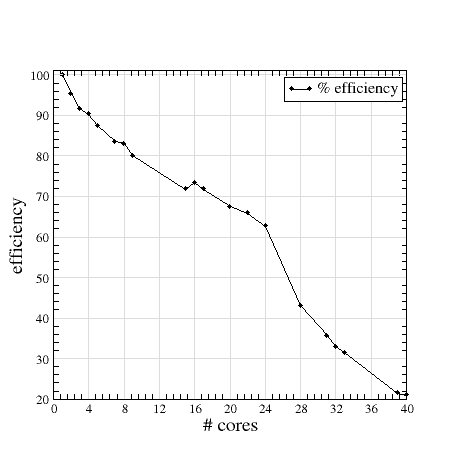
\includegraphics[width=0.45\textwidth]{efficiency}
    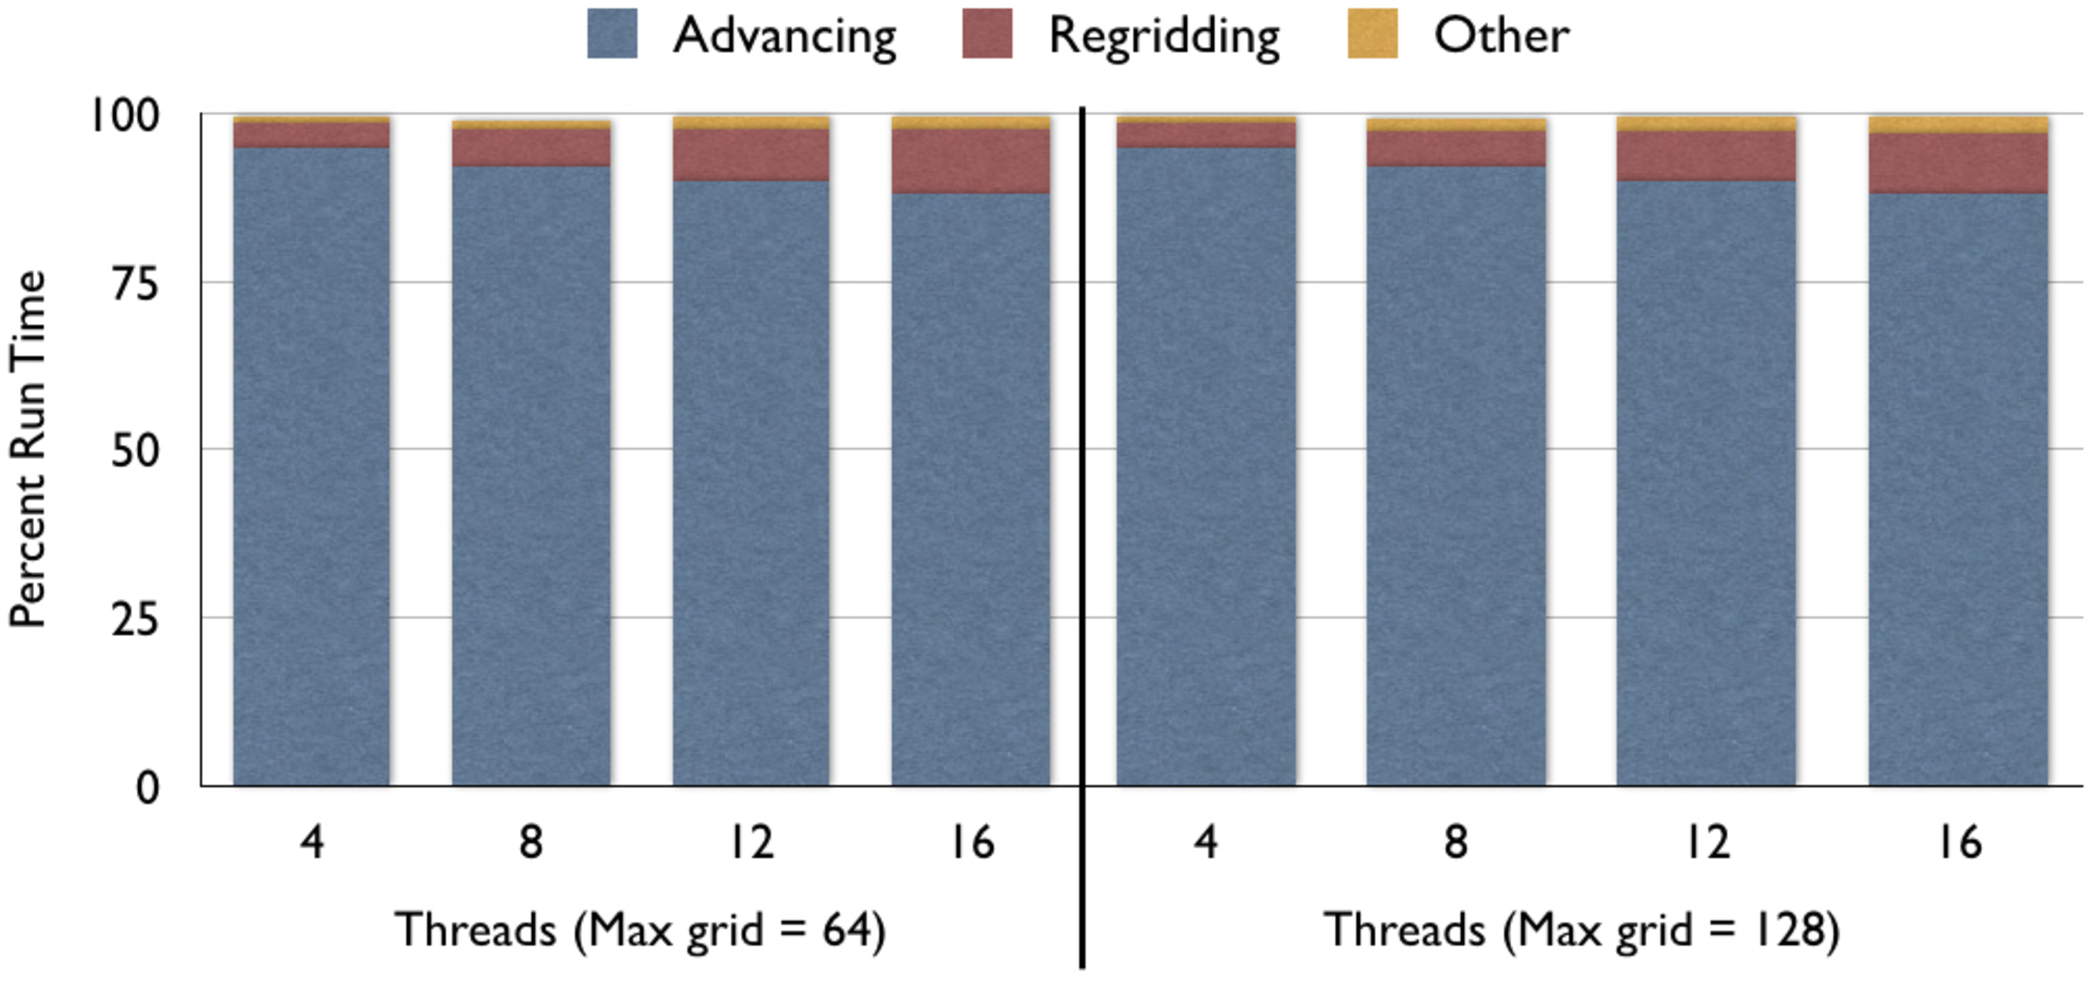
\includegraphics[width=0.45\textwidth]{weak_scaling}
    \caption{Scaling results for an \amrclaw example demonstrating a
    shock-bubble interaction in the Euler equations of compressible
    gas-dynamics.}
    \label{fig:amr_scaling}
\end{figure}

The parallelization of \amrclaw and \geoclaw assumes multi-core machines for the
target architecture.  \pyclaw, on the other hand, does not include AMR but uses
MPI via PETSc to achieve parallelism on distributed memory machines that scale
to tens of thousands of cores (see \cref{sec:pyclaw}). Other frameworks exist,
most notably \forestclaw \cite{Burstedde:we}, which are being developed in
parallel with \amrclaw, that provide scalable AMR calculations on large
distributed
memory machines.

